\documentclass[11pt,a4paper]{article}

\usepackage[utf8]{inputenc}
\usepackage[T1]{fontenc}
\usepackage{lmodern}
\usepackage[margin=2.2cm]{geometry}
\usepackage{microtype}
\usepackage{booktabs}
\usepackage{tabularx}
\usepackage{array}
\usepackage{enumitem}
\usepackage[table]{xcolor}
\usepackage{siunitx}
\usepackage{tikz}
\usetikzlibrary{positioning,arrows.meta,calc,fit}
\usepackage{caption}
\usepackage{needspace}
\usepackage{float}
\usepackage[hidelinks]{hyperref}

\sisetup{range-phrase = --, range-units = single}
\setlist{itemsep=2pt, topsep=4pt}
\captionsetup{font=small, labelfont=bf}
\newcolumntype{L}{>{\raggedright\arraybackslash}X}
\newcommand{\pin}[1]{\texttt{#1}}
\newcommand{\est}{\textsuperscript{\,est.}}

\definecolor{accent}{HTML}{2F6DB5}
\definecolor{band}{HTML}{EEF2F7}

\title{\textbf{Proposal: Programmable 8\,Gb/s CTLE}\\[4pt]
\large Chipalooza Challenge \#4 \textperiodcentered{} SkyWater SKY130}
\author{}
\date{November 2026}

\begin{document}
\maketitle

%--------------------------------------------------------------------
\section{IP block type and summary}

\textbf{IP block:} a digitally programmable continuous-time linear
equalizer (CTLE) for chip-to-chip serial links up to \SI{8}{Gb/s}
(PCIe~3.0, \SI{4}{GHz} Nyquist) in SkyWater SKY130.

A 3-bit control selects 8 equalization levels covering \SIrange{10}{20}{dB}
of channel loss at Nyquist. The block takes a single-ended input, converts it
on-chip to differential, equalizes it in two stages, and drives a
\SI{50}{\ohm}-matched differential output off-chip.

\textbf{Why it is useful in an SoC.} Every receiver of a fast serial link
(PCIe, USB\,3, SATA, Ethernet, DisplayPort) starts with a CTLE. Stand-alone
programmable CTLEs are also sold as linear redrivers to extend channel
reach. The open SKY130 IP set has no wireline receive equalizer yet. This
block is a reusable first building block toward an open-source serial-link
receiver, alongside the comparators and PLLs already available.

The core reuses a two-stage SKY130 CTLE the team
has already designed and verified post-layout at \SI{8}{Gb/s}. This
proposal makes the boost programmable over a wider range and adds the input
and output circuits needed to test it through the Chipalooza harness.

%--------------------------------------------------------------------
\section{I/O list}

The three high-speed signals use the three dedicated pads, since
\SI{4}{GHz} signals cannot pass through the shared analog mux. The block uses
no shared analog lines. \pin{OUTP} and \pin{OUTN} are the test ports.
Power-down is handled by the harness slot power switch; the block has no
enable pin.

\begin{table}[h]
\centering\small
\caption{I/O list.}
\begin{tabularx}{\linewidth}{@{}l l l l L@{}}
\toprule
Signal & Type & Dir & Harness resource & Function \\
\midrule
\pin{IN}        & Analog, high speed & In  & Dedicated pad 0 & Single-ended data input, AC-coupled off-chip \\
\pin{OUTP}      & Analog, high speed (test port) & Out & Dedicated pad 1 & Equalized output, positive, into \SI{50}{\ohm} \\
\pin{OUTN}      & Analog, high speed (test port) & Out & Dedicated pad 2 & Equalized output, negative, into \SI{50}{\ohm} \\
\pin{CTRL[2:0]} & Digital, static    & In  & Control inputs 0--2 & Boost code \\
\pin{IBIAS}     & Analog, DC         & In  & Harness reference current 0 & Mirrored on-chip to all stages \\
\pin{VPWR}, \pin{VGND} & Power       & --- & Slot supply & \SI{1.8}{V}, about \SI{16}{mA} (Section~\ref{sec:spec}) \\
\bottomrule
\end{tabularx}
\end{table}

%--------------------------------------------------------------------
\section{Functional description and architecture}

The signal enters on one pad, becomes differential on-chip, is equalized
in two stages and leaves through two \SI{50}{\ohm}-matched pads. The block
is analog with static digital configuration inputs: no clock and no
synthesized logic.

\begin{figure}[h]
\centering
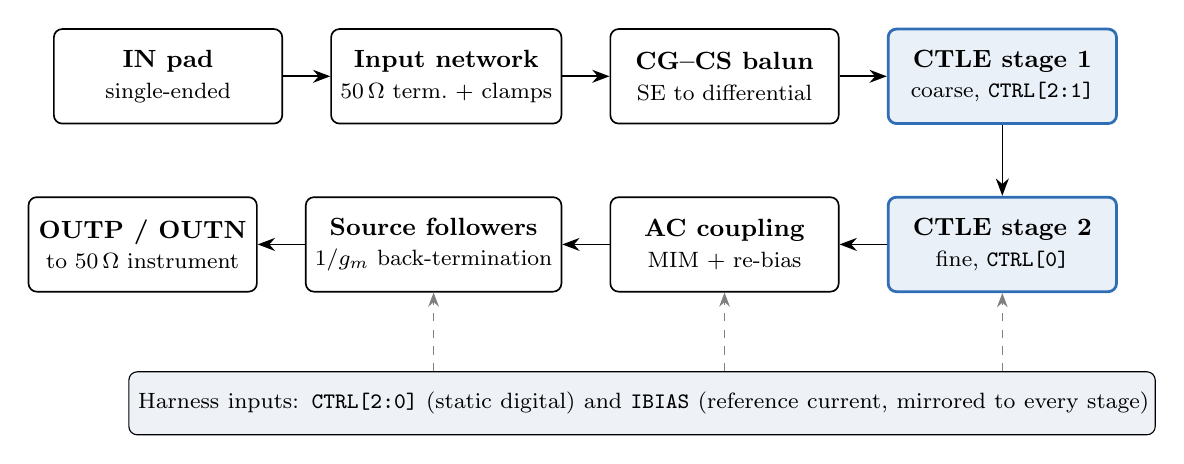
\begin{tikzpicture}[
  font=\small,
  blk/.style={draw, rounded corners=3pt, minimum width=29mm, minimum height=12mm, align=center, line width=0.6pt},
  core/.style={blk, draw=accent, fill=accent!10, line width=1pt},
  sig/.style={-{Stealth[length=2.2mm]}, line width=0.6pt},
  ctl/.style={-{Stealth[length=1.8mm]}, dashed, line width=0.5pt, draw=gray}
]
  \node[blk]  (in)   {\textbf{IN pad}\\ \footnotesize single-ended};
  \node[blk,  right=6mm of in]   (net)  {\textbf{Input network}\\ \footnotesize \SI{50}{\ohm} term.\ + clamps};
  \node[blk,  right=6mm of net]  (bal)  {\textbf{CG--CS balun}\\ \footnotesize SE to differential};
  \node[core, right=6mm of bal]  (s1)   {\textbf{CTLE stage 1}\\ \footnotesize coarse, \pin{CTRL[2:1]}};
  \node[core, below=9mm of s1]   (s2)   {\textbf{CTLE stage 2}\\ \footnotesize fine, \pin{CTRL[0]}};
  \node[blk,  left=6mm of s2]    (ac)   {\textbf{AC coupling}\\ \footnotesize MIM + re-bias};
  \node[blk,  left=6mm of ac]    (sf)   {\textbf{Source followers}\\ \footnotesize $1/g_m$ back-termination};
  \node[blk,  left=6mm of sf]    (out)  {\textbf{OUTP / OUTN}\\ \footnotesize to \SI{50}{\ohm} instrument};
  \draw[sig] (in) -- (net);
  \draw[sig] (net) -- (bal);
  \draw[sig] (bal) -- (s1);
  \draw[sig] (s1) -- (s2);
  \draw[sig] (s2) -- (ac);
  \draw[sig] (ac) -- (sf);
  \draw[sig] (sf) -- (out);
  \node[draw, rounded corners=3pt, fill=band, minimum height=8mm, text width=128mm, align=center,
        below=10mm of $(sf.south)!0.5!(ac.south)$, xshift=8mm] (harness)
        {\footnotesize Harness inputs: \pin{CTRL[2:0]} (static digital) and \pin{IBIAS} (reference current, mirrored to every stage)};
  \foreach \n in {sf, ac, s2} \draw[ctl] (harness.north -| \n.south) -- (\n.south);
\end{tikzpicture}
\caption{Signal path: single-ended in, equalized \SI{50}{\ohm} differential out. Solid arrows carry the signal; dashed arrows are static control and bias.}
\label{fig:block}
\end{figure}

\begin{enumerate}
\item \textbf{Input network.} Single-ended input on a dedicated pad, with
  on-chip \SI{50}{\ohm} termination and core-side clamps for the overvoltage
  protection \SI{1.8}{V} devices need behind a pad.
\item \textbf{Active balun.} A common-gate/common-source pair turns the
  single-ended input into a balanced differential signal. The common-gate
  device sets the \SI{50}{\ohm} input match.
\item \textbf{CTLE core.} Two cascaded source-degenerated differential
  stages with resistor loads. Fixed MIM degeneration capacitors bridge the
  source nodes directly, with no switch in series. Binary-weighted
  degeneration-resistor banks set the boost; their switches sit at the
  differential virtual ground so their resistance and capacitance stay out
  of the signal path. Stage~1 takes the two coarse bits
  ($\approx\SI{2.9}{dB}$ steps), stage~2 the fine bit
  ($\approx\SI{1.4}{dB}$). A switched tail-current bank holds the peak gain
  level across codes.
\item \textbf{Output drivers.} The CTLE output is AC-coupled through a MIM
  capacitor and re-biased for headroom with one NMOS source follower per side.
\item \textbf{Control and bias.} \pin{CTRL[2:0]} drives the resistor and
  tail banks directly: stage~1 takes the two coarse bits, stage~2 the
  fine bit. \pin{IBIAS} from the harness is
  mirrored to all stages.
\end{enumerate}

\textbf{Why a single-ended input.} The harness provides at most three
dedicated pads, and the shared analog lines are multiplexed and not suited
to \SI{4}{GHz} signals. A fully differential test of the CTLE would need four
high-speed pads (INP, INN, OUTP, OUTN), one more than is available. Three
ways to fit were considered:
\begin{itemize}
\item \textbf{Differential input, output measured by on-chip amplitude
  detectors} read as DC voltages on the shared lines. This fits, but gives
  no S-parameters or eye at the output, and every gain reading depends on
  how well the detectors match.
\item \textbf{Differential input, single-ended output.} This also uses three
  pads, but puts the conversion where the signal is largest and already
  equalized, and it must drive \SI{50}{\ohm} at \SI{4}{GHz}.
\item \textbf{Single-ended input, on-chip balun, differential output
  (chosen).} The conversion happens where the signal is small, and the
  common-gate device of the balun also sets the \SI{50}{\ohm} input match.
  The CTLE core stays fully differential, and the output can be measured
  directly with a network analyzer and a sampling scope.
\end{itemize}
The balun adds gain and phase imbalance, some power and some noise in front
of the core. Its response cancels in the measurement: dividing each code's
response by that of code 000 removes the balun, output buffers and
package, leaving the boost of the CTLE core. The balun and output drivers exist
for test access; the reusable IP is the differential CTLE core.

%--------------------------------------------------------------------
\section{Target specification}
\label{sec:spec}

The block equalizes \SIrange{10}{20}{dB} of channel loss at \SI{4}{GHz} in
8 codes. Conditions unless noted: $V_\mathrm{PWR} =
\SI{1.8}{V}$, TT, \SI{27}{\celsius}, post-layout, pad and package models
included. Values marked est.\ are first estimates to be fixed at the
schematic review.

\begin{table}[h]
\centering\small
\caption{Target specification.}
\label{tab:spec}
\begin{tabularx}{\linewidth}{@{}L r r r l L@{}}
\toprule
Parameter & Min & Typ & Max & Unit & Notes \\
\midrule
Supply voltage, $V_\mathrm{PWR}$ & 1.62 & 1.8 & 1.98 & V & \\
Data rate & --- & 8 & --- & Gb/s & NRZ, UI = \SI{125}{ps} \\
Boost step & 1.0 & 1.43 & 2.0 & dB & \\
Input return loss, S11 & 10 & --- & --- & dB & \SIrange{0}{2}{GHz}; reported to \SI{4}{GHz} \\
Output return loss, S22 & 10 & --- & --- & dB & \SIrange{0}{4}{GHz}, each output \\
Eye height at CTLE core output & 225 & 250 & 275 & mVpp,diff & Matched code and channel; simulation \\
Eye width & 0.35 & --- & --- & UI & PRBS7 \\
Supply current & --- & 16 & 20 & mA & \\
Temperature & $-40$ & 27 & 110 & \si{\celsius} & Post-layout PVT \\
\bottomrule
\end{tabularx}
\end{table}

%--------------------------------------------------------------------
\section{Test plan}

The block is validated in two steps: simulation tests before tapeout, then
physical tests on the fabricated chip.

\subsection{Simulation tests}

Every specification in Section~\ref{sec:spec} is signed off in post-layout
PVT simulation with open-source tools only (Xschem, ngspice, Magic, KLayout,
Netgen, CACE) using the Chipalooza template flow.

\begin{table}[h]
\centering\small
\caption{Simulation tests.}
\begin{tabularx}{\linewidth}{@{}l L l@{}}
\toprule
Check & What it covers & Pass criterion \\
\midrule
AC response, all 8 codes & Boost and peak frequency & Table~\ref{tab:spec} \\
PRBS7 eye, matched code per channel & Eye at the CTLE core output (\SI{10}{dB} and \SI{20}{dB} channels) & Table~\ref{tab:spec} \\
S11 and S22 & With pad, ESD, bond-wire and package models & $\geq\SI{10}{dB}$ in band \\
Monte Carlo ($\geq 100$ runs) & Offset, balun mismatch, boost spread; schematic and extracted & Table~\ref{tab:spec} \\
PVT & ss, ff, sf, fs $\times$ 1.62/1.98\,V $\times$ $-40$/27/110\,\si{\celsius} & Table~\ref{tab:spec} \\
Layout checks & Magic and KLayout DRC, Netgen and KLayout LVS, Magic extraction & Extraction Clean \\
\bottomrule
\end{tabularx}
\end{table}

\subsection{Physical tests}

The chip is measured directly through its pads: S-parameters on a network
analyzer, and eye diagrams with an \SI{8}{Gb/s} PRBS source and a sampling
scope. If requested equipment list can be sent seperatly with detail.

\begin{enumerate}
\item \textbf{Power-up.} Supply current per code and output common-mode levels.
\item \textbf{Return loss.} S11 at \pin{IN} and S22 at each output,
  \SI{10}{MHz} to \SI{6}{GHz}.
\item \textbf{Frequency response per code.} Single-ended-to-differential
  transmission (mixed-mode S-parameters) for all 8 codes. The ratio of each
  code's response to code 000 cancels the balun, output buffers and
  package, so the boost of the CTLE core comes out directly.
\item \textbf{Eye diagrams.} PRBS7 and PRBS15 at \SI{8}{Gb/s} through
  \SI{10}{dB} and \SI{20}{dB} test channels, each with its matched code; eye
  height and width at the output pads. The input amplitude is reduced for
  low-loss channels to stay inside the linear range.
\end{enumerate}

All measured data and scripts will be published in the repository.

%--------------------------------------------------------------------
\Needspace{26\baselineskip}
\section{Risks and mitigations}

\begin{table}[H]
\centering\small
\caption{Risks and mitigations.}
\begin{tabularx}{\linewidth}{@{}>{\raggedright\arraybackslash}p{3.3cm} L L@{}}
\toprule
Risk & Effect & Mitigation \\
\midrule
Pad, bond-wire and package parasitics & $\sim$\SI{2}{nH} with $\sim$\SI{1}{pF} resonates near \SI{3.6}{GHz}; S11 and S22 degrade above \SI{2}{GHz} & S11/S22 specified over \SIrange{0}{2}{GHz} only; pad and package model in every testbench; \SI{4}{GHz} boost measured through de-embedding \\
Active-balun imbalance & Gain and phase mismatch turn into common-mode signal and lower the differential eye & Matched CG and CS devices in a common-centroid layout; imbalance swept over PVT and Monte Carlo before the schematic review \\
Output-to-input coupling & Feedback from the \SI{50}{\ohm} output drivers to the input can cause peaking or oscillation & \pin{IN} kept apart from \pin{OUTP}/\pin{OUTN} in the layout; separate supply straps for drivers and core; stability checked with the pad model in the loop \\
Follower headroom at large input & At full CTLE swing the source followers can cut off (about \SI{\pm4.7}{mA} demanded at \SI{10}{dB} boost) & Specified linear input range; follower bias sized with margin; large-signal PRBS sweep at every code \\
Slot supply current & $\sim$\SI{16}{mA} may exceed what the slot power switch allows & Supply current kept within the slot budget; tail currents trimmable through \pin{IBIAS} \\
Realized boost below the ideal formula & Parasitic capacitance at the degeneration nodes lowers the zero-pole spacing; codes compress & Boost extracted from post-layout netlists at every code; range designed with headroom past \SI{20}{dB} \\
\bottomrule
\end{tabularx}
\end{table}

\end{document}
